%%%%%%%%%%%%% local definitions %%%%%%%%%%%%%%%%%%%%%
% This allows for switching between one column and two column (cms@external) layouts
% The widths should  be modified for your particular figures. You'll need additional copies if you have more than one standard figure size.
\newlength\cmsFigWidth
\ifthenelse{\boolean{cms@external}}{\setlength\cmsFigWidth{0.85\columnwidth}}{\setlength\cmsFigWidth{0.4\textwidth}}
\ifthenelse{\boolean{cms@external}}{\providecommand{\cmsLeft}{top}}{\providecommand{\cmsLeft}{left}}
\ifthenelse{\boolean{cms@external}}{\providecommand{\cmsRight}{bottom}}{\providecommand{\cmsRight}{right}}

%%%%%%%%%%%%%%%  Title page %%%%%%%%%%%%%%%%%%%%%%%%
\cmsNoteHeader{PFCalEE} % This is over-written in the CMS environment: useful as preprint no. for export versions
% >> Title: please make sure that the non-TeX equivalent is in
PDFTitle below \title{Simulation and performance studies of a highly
granular electromagnetic calorimeter for the phase-II upgrade of the
CMS endcap region.}

% >> Authors
%Author is always "The CMS Collaboration" for PAS and papers, so author, etc, below will be ignored in those cases
%For multiple affiliations, create an address entry for the combination
%To mark authors as primary, use the \author* form
\address[IC]{Imperial College London (UK)}
\author[IC]{Paul Dauncey, Anne-Marie Magnan}    
\address[CERN]{CERN}
\author[CERN]{Pedro Silva}
\address[UCLA]{UCLA}
\author[UCLA]{Valeri Andreeiv}


% >> Date
% The date is in yyyy/mm/dd format. Today has been
% redefined to match, but if the date needs to be fixed, please write it in this fashion.
% For papers and PAS, \today is taken as the date the head file (this one) was last modified according to svn: see the RCS Id string above.
% For the final version it is best to "touch" the head file to make sure it has the latest date.
\date{\today}

% >> Abstract
% Abstract processing:
% 1. **DO NOT use \include or \input** to include the abstract: our abstract extractor will not search through other files than this one.
% 2. **DO NOT use %**                  to comment out sections of the abstract: the extractor will still grab those lines (and they won't be comments any longer!).
% 3. For PASs: **DO NOT use tex macros**         in the abstract: CDS MathJax processor used on the abstract doesn't understand them _and_ will only look within $$. The abstracts for papers are hand formatted so macros are okay.
\abstract{

A highly granular Si-Pb sampling calorimeter is proposed to replace
the existing endcap calorimeter during the Phase-II upgrade of the CMS
detector. This note concentrates on the simulation and physics
performance studies for the electromagnetic part. A standalone
simulation of a small detector unit in Geant4 is used to optimise the
design, and extract first information about electromagnetic showers,
e.g.  energy resolution, shower profile, position resolution. A
digitisation procedure is also put into place to add "reality" to the
simulation. All studies are repeated in the context of the high
pile-up environment expected from the high-luminosity LHC. The whole
chain has also been ported to CMSSW with the simulation of the full
detector.

}

% >> PDF Metadata
% Do not comment out the following hypersetup lines (metadata). They will disappear in NODRAFT mode and are needed by CDS.
% Also: make sure that the values of the metadata items are sensible and are in plain text:
% (1) no TeX! -- for \sqrt{s} use sqrt(s) -- this will show with extra quote marks in the draft version but is okay).
% (2) no %.
% (3) No curly braces {}.
\hypersetup{%
pdfauthor={A.-M. Magnan, P. Silva},%
pdftitle={PFCalEE},%
pdfsubject={CMS},%
pdfkeywords={CMS, upgrade, HGCAL}}

\maketitle %maketitle comes after all the front information has been supplied
% >> Text
%%%%%%%%%%%%%%%%%%%%%%%%%%%%%%%%  Begin text %%%%%%%%%%%%%%%%%%%%%%%%%%%%%
%% **DO NOT REMOVE THE BIBLIOGRAPHY** which is located before the appendix.
%% You can take the text between here and the bibiliography as an example which you should replace with the actual text of your document.
%% If you include other TeX files, be sure to use "\input{filename}" rather than "\input filename".
%% The latter works for you, but our parser looks for the braces and will break when uploading the document.
%%%%%%%%%%%%%%%

\tableofcontents
 
% AM
\section{Introduction}
\label{sec:intro}
% AM
\section{Setup}
\label{sec:setup}

Two different setups are used, in order to systematically provide an
independant cross check of the results:
\begin{itemize}
\item standalone simulation of a detector with a transverse size of $20 \times 20$cm$^2$ and 30 layers.
\item full geometry of the final detector in CMSSW.
\end{itemize}

For the standalone simulation, two different analyses are also run in
parallel and cross-checking each others systematically.

\subsection{The standalone simulation setup}
\label{sec:standalone}

This setup is used for three different purposes: provide a quick
handle to optimise the design parameters (see
section~\ref{sec:optim}), extract performance results in ideal
conditions, and cross-check the performances in pileup conditions with
the CMSSW setup. The code is available in git under the following
repository: \url{https://github.com/pfs/PFCal/}.

\subsubsection{Geant4 setup}

The detector construction is made of 30 sampling sections, each with
the material detailed in table~\ref{tab:samplSec}.

\begin{table}[h!]
 \begin{center}
\caption{\label{tab:samplSec} Thicknesses (in mm) for the different materials, per layer}
\begin{tabular}{|l|c|c|c|c|c|}
\hline
Layers & Pb & Cu & Si & PCB & Air \\
\hline
0-9  & 1.63 & 3 & 0.2 & 1 & 2 \\
10-19 & 3.32 & 3 & 0.2 & 1 & 2 \\
20-29 & 5.56 & 3 & 0.2 & 1 & 2 \\
\hline
\end{tabular}
\end{center}
\end{table}

Figure~\ref{fig:g4vis} shows an event display of a 50 GeV electron
shower in two different geometries: a uniform 26 layers of 1 X$_0$
each (left) and the baseline geometry detailed in
table~\ref{tab:samplSec} (right).

\begin{figure}[h!]
  \begin{center}
    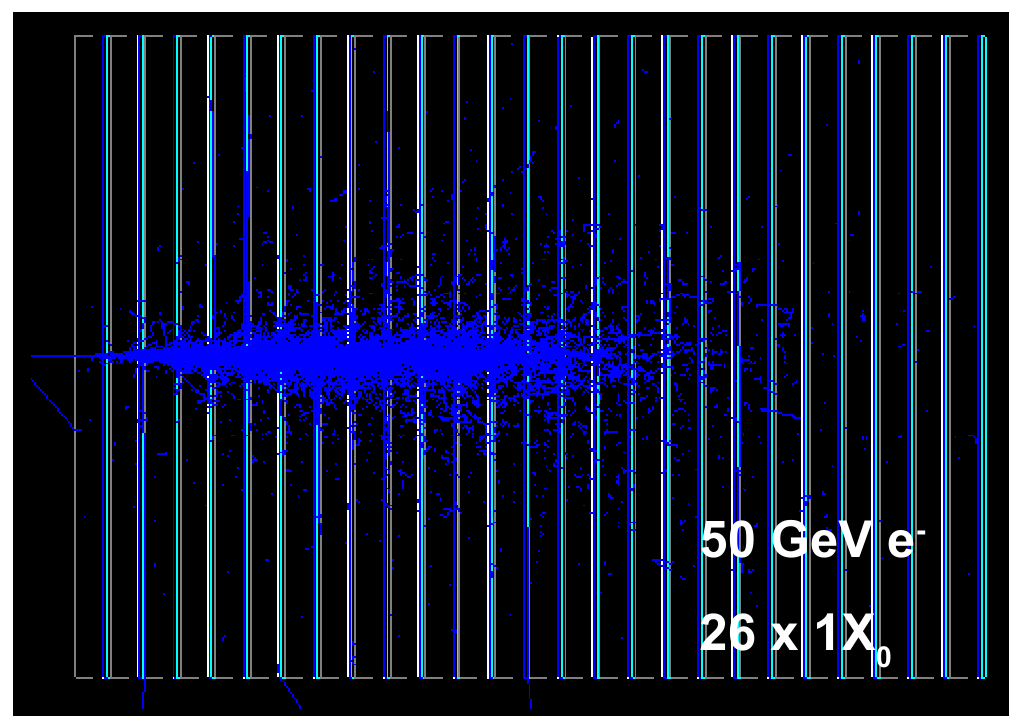
\includegraphics[width=\cmsFigWidth]{figures/e_50GeV_uniform_26x0.png}
    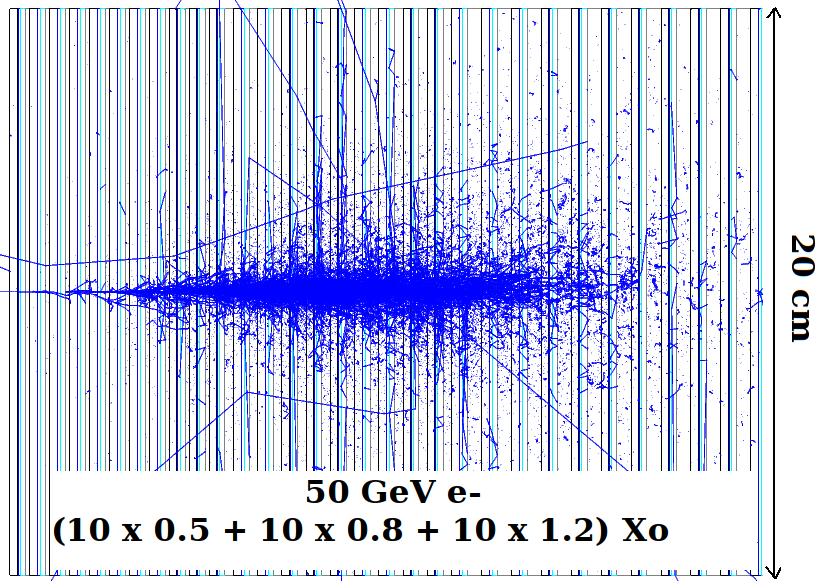
\includegraphics[width=\cmsFigWidth]{figures/e_50GeV_concept_v3.png}
    \caption{Event displays of a 50 GeV electron showers in the
      standalone simulation. Left: uniform 26 layers of 1 X$_0$
      each. Right: 30 layers in three blocks of different
      thicknesses. Electron deposits are shown in blue. Photons have
      been hidden for better visibility.}
    \label{fig:g4vis}
  \end{center}
\end{figure}

The simulation uses the QGSP\_FTFP\_BERT physics list, with the default cuts
for electrons, positrons and photons reduced to 10\,$\mu$m in the
silicon. The default elsewhere is 1\,mm. With 700\,$\mu$m in Si,
a 420 keV (5.8 keV) electron (photon) would deposit all its energy in
one step. With the reduced 10\,$\mu$m, the energy threshold is 32 keV
for electrons, and 990 eV for photons.


\subsubsection{Energy calibration and resolution}

Different methods are used to measure the total energy:
\begin{itemize}
\item raw energy: simply the sum of the energy deposited in Geant4 in
  the silicon in the full detector volume (30 layers of $20 \times
  20$\,cm$^2$).
\item weighted energy: sum of the energy deposited in the Si, but
  weighted differently according to which sampling section they belong
  to. Simplest weights are the ratio of sampling thicknesses in X$_0$,
  i.e. 1 for layers 0-9, 0.8/0.5 for layers 10-19 and 1.2/0.5 for
  layers 20-29. Weights can also be optimised to minimise the energy
  resolution for all energies.
\item Fit of the shower profile: allowing for example to recover the
  shower leakage for higher energies.
\end{itemize}

For the first two methods, the total energy is fitted, per incoming
energy generated, by a gaussian. The mean is used for calibration, and
the resolution is defined as the ratio of the width over the mean.

The calibration curve is shown in Figure~\ref{fig:eCalib} left, for
single electrons. Figure~\ref{fig:eCalib} right, shows the energy
resolution as a function of the incoming energy. For incoming energies
below 150 GeV, 2500 events have been generated, and 1250 above.

%@TODO replace with Pedro's plots with all 3 methods in.
\begin{figure}[h!]
  \begin{center}
    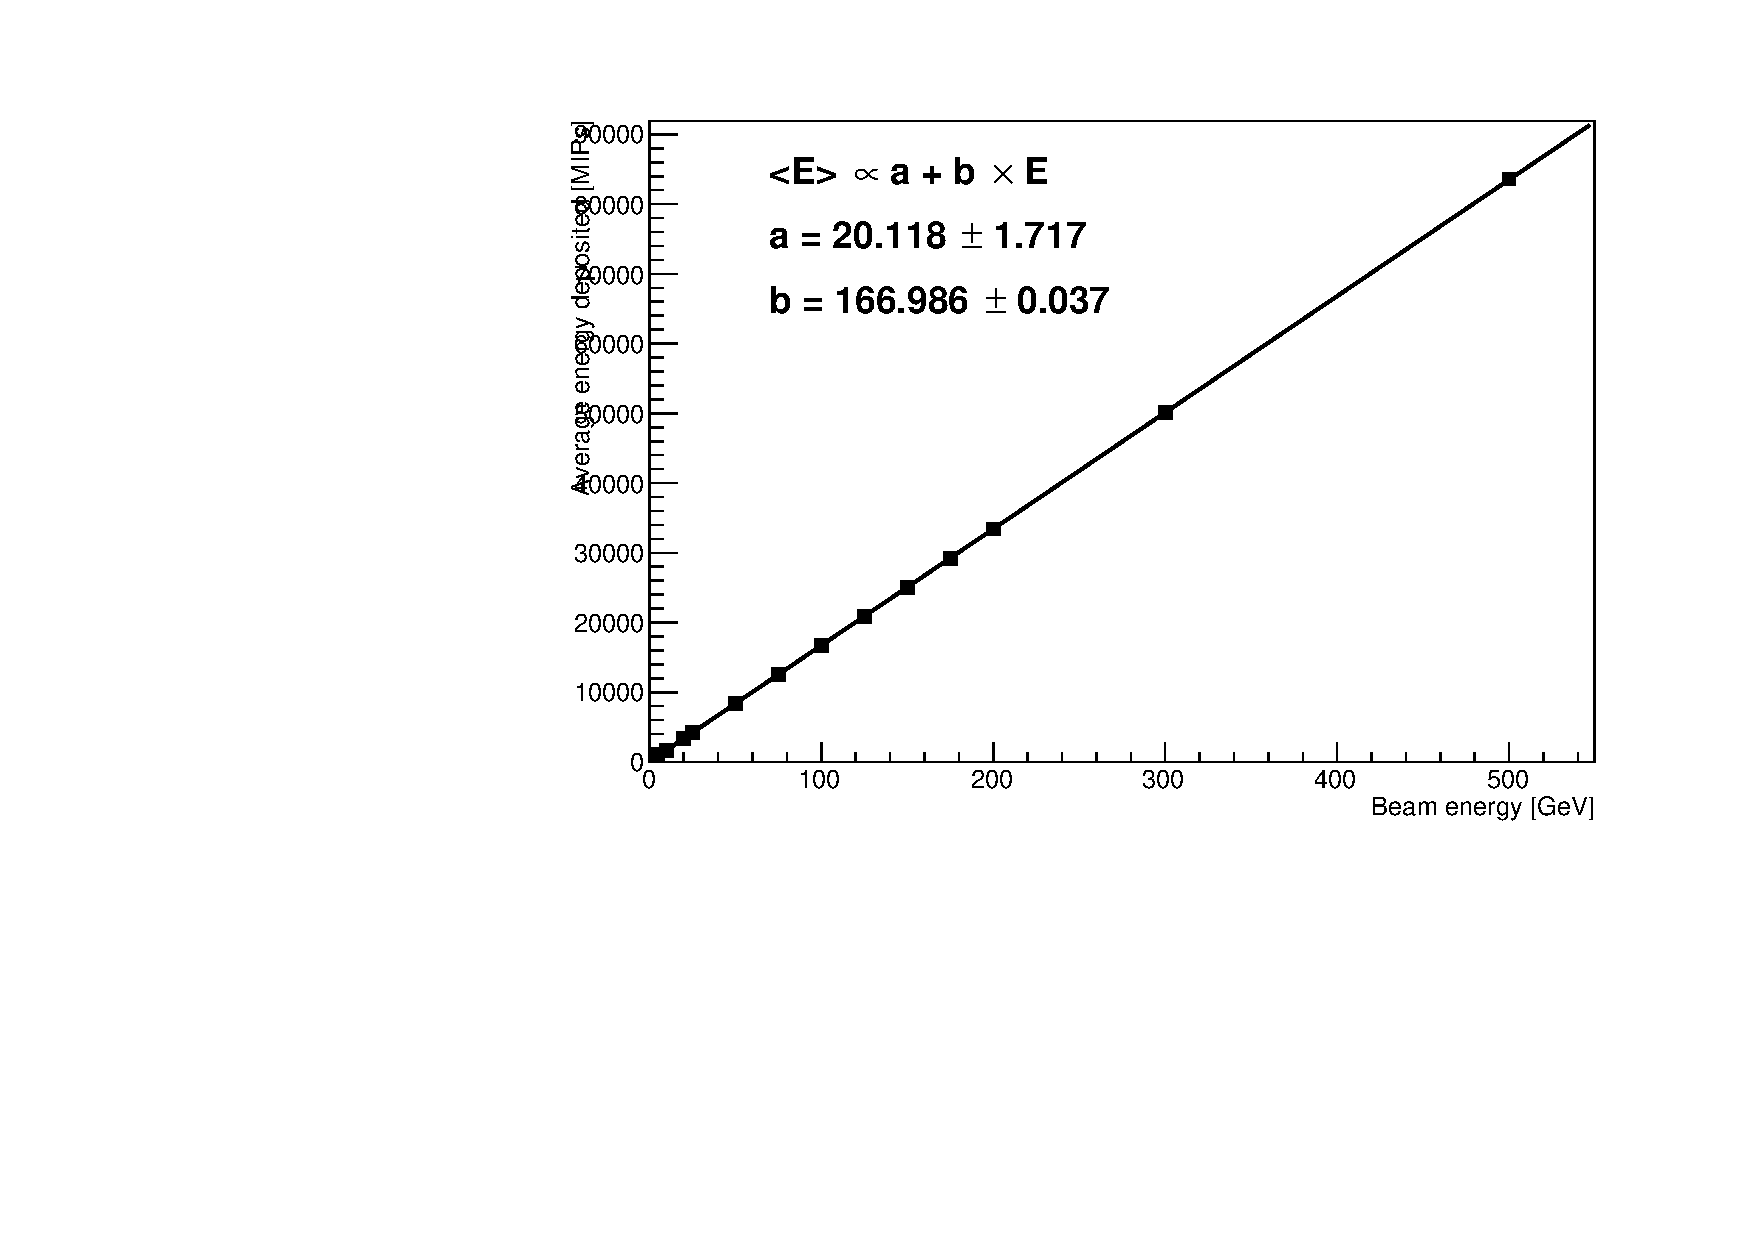
\includegraphics[width=\cmsFigWidth]{figures/e_calibFit.pdf}
    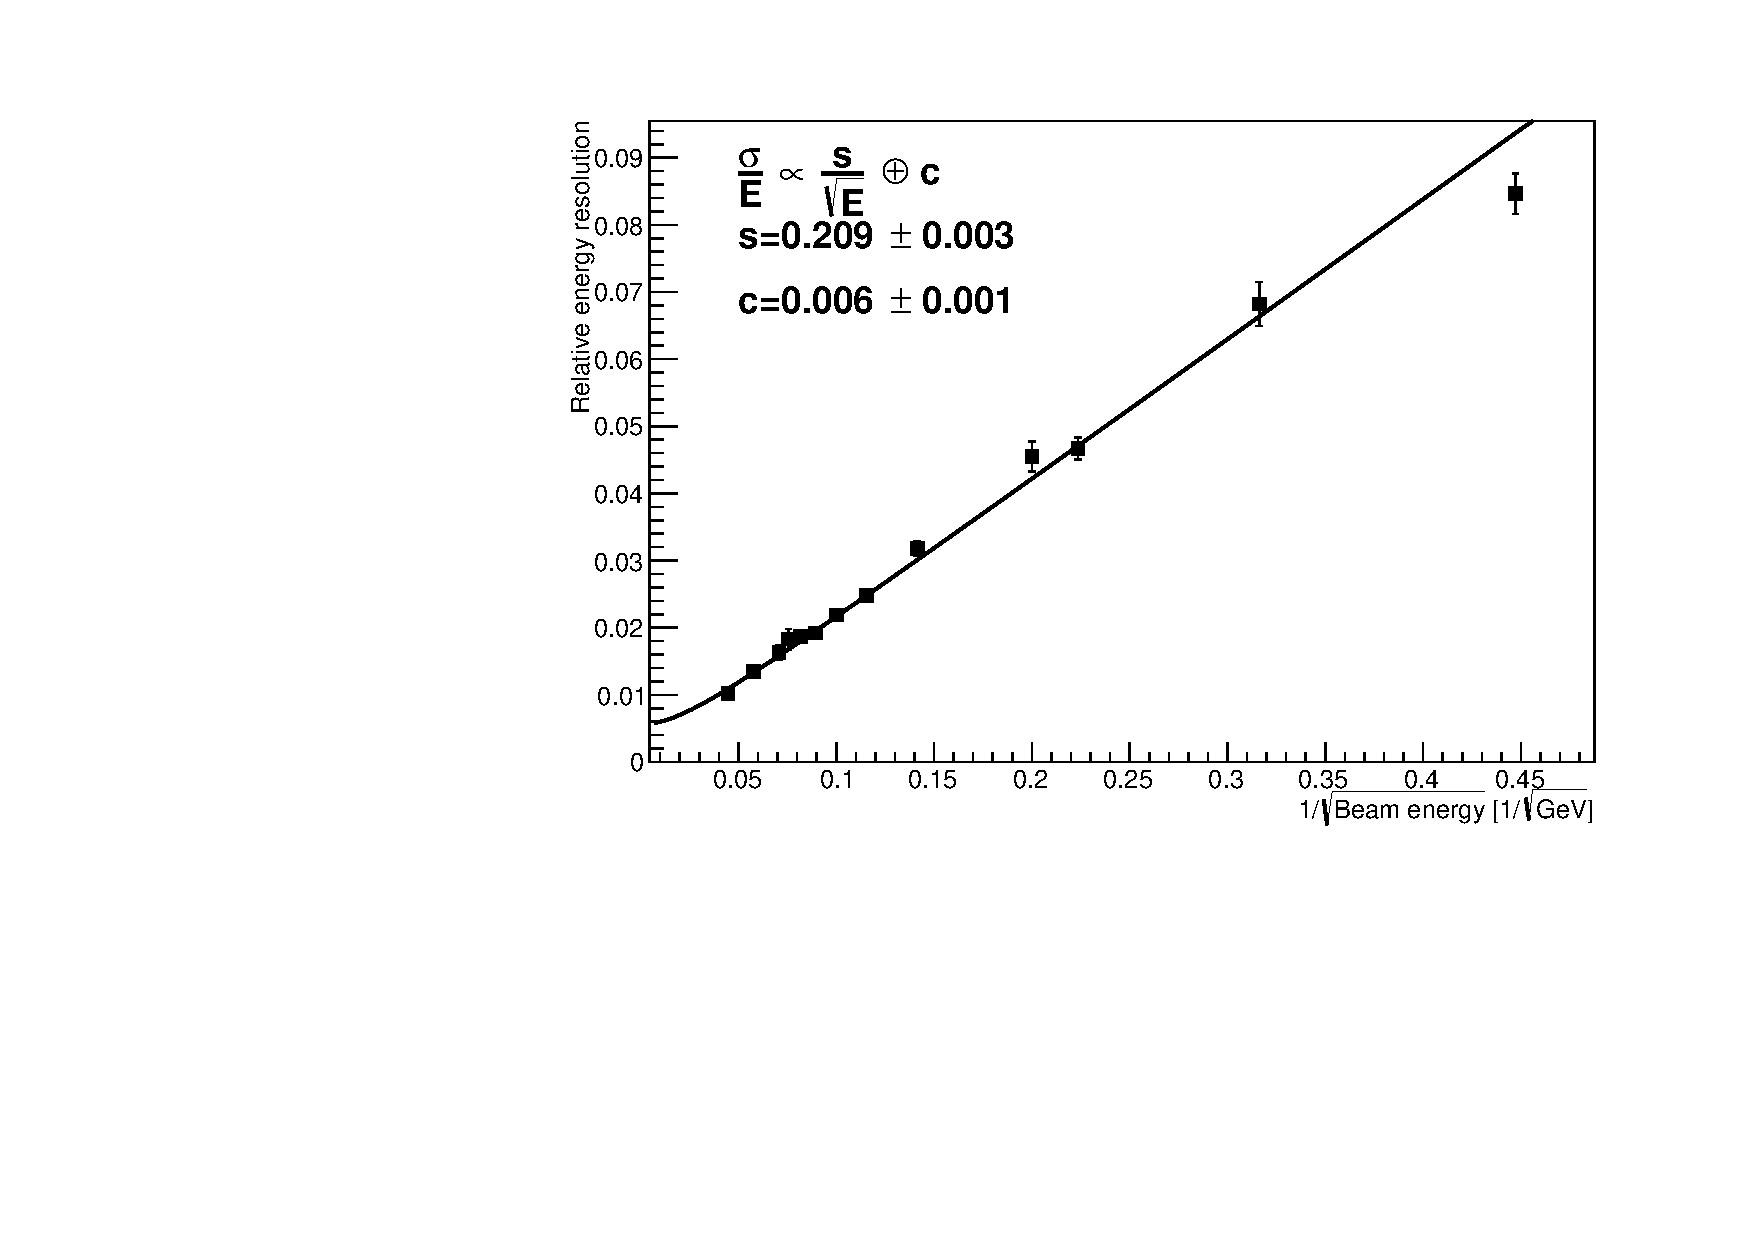
\includegraphics[width=\cmsFigWidth]{figures/e_resoFit.pdf}
    \caption{Reconstructed energy as a function of the generated
      energy E (left) and energy resolution as a function of
      $\frac{1}{\sqrt{E}}$ (right), for single electron events.}
    \label{fig:g4vis}
  \end{center}
\end{figure}



% Pedro
\section{Setup in CMSSW}
\label{sec:cmssw}

\subsection{Geometry in CMSSW}

\subsection{SimHits}

\subsection{Event displays}

\subsection{RecHits}

\subsection{PandoraPFA}

% Pedro
%
%
%
\clearpage
\section{Optimisation of the design}
\label{sec:optim}

\FIXME{Add introduction}

\FIXME{Varying the Silicon width test}

\FIXME{Varying the sampling fractions test}

\FIXME{Varying the absorber material test}



\begin{figure}[h!]
  \begin{center}
  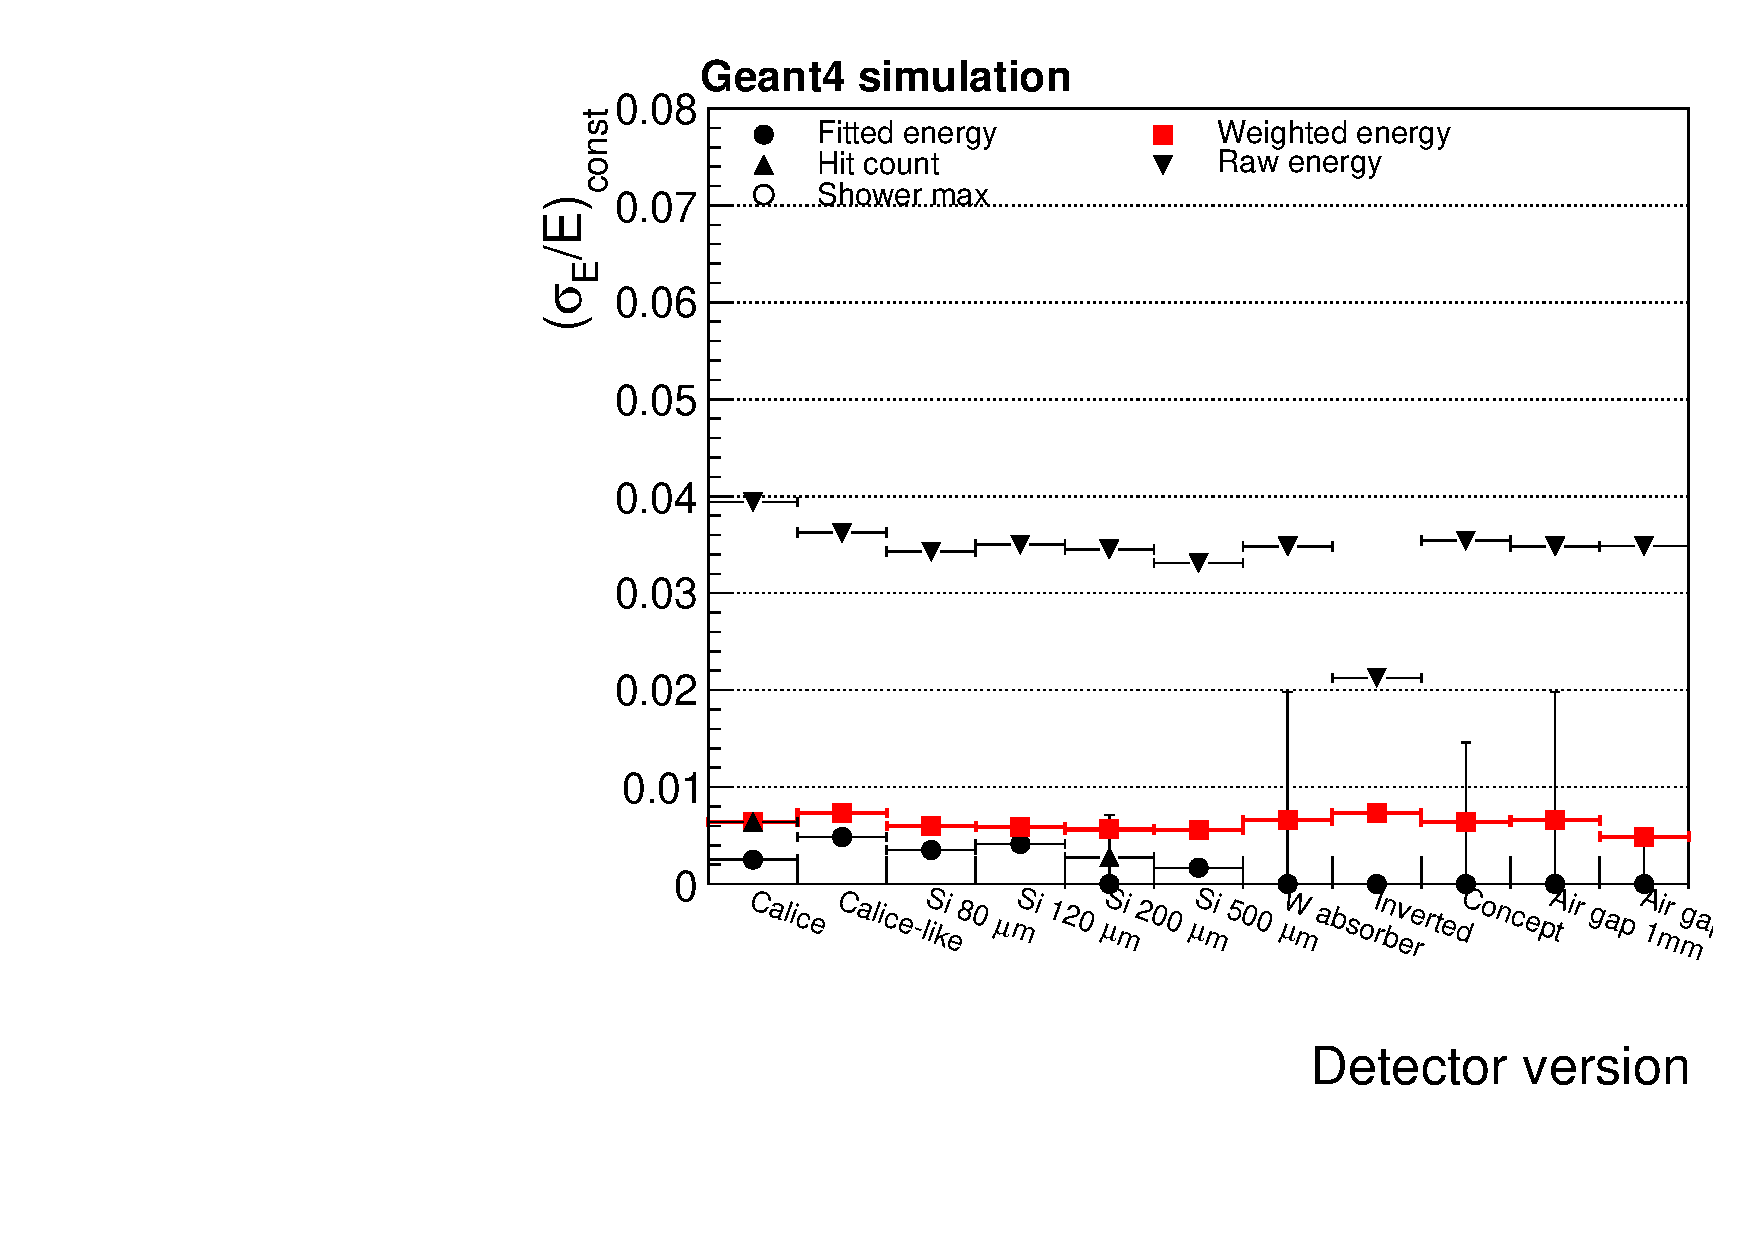
\includegraphics[width=0.75\textwidth]{figures/ResolutionSummary_const}\\
  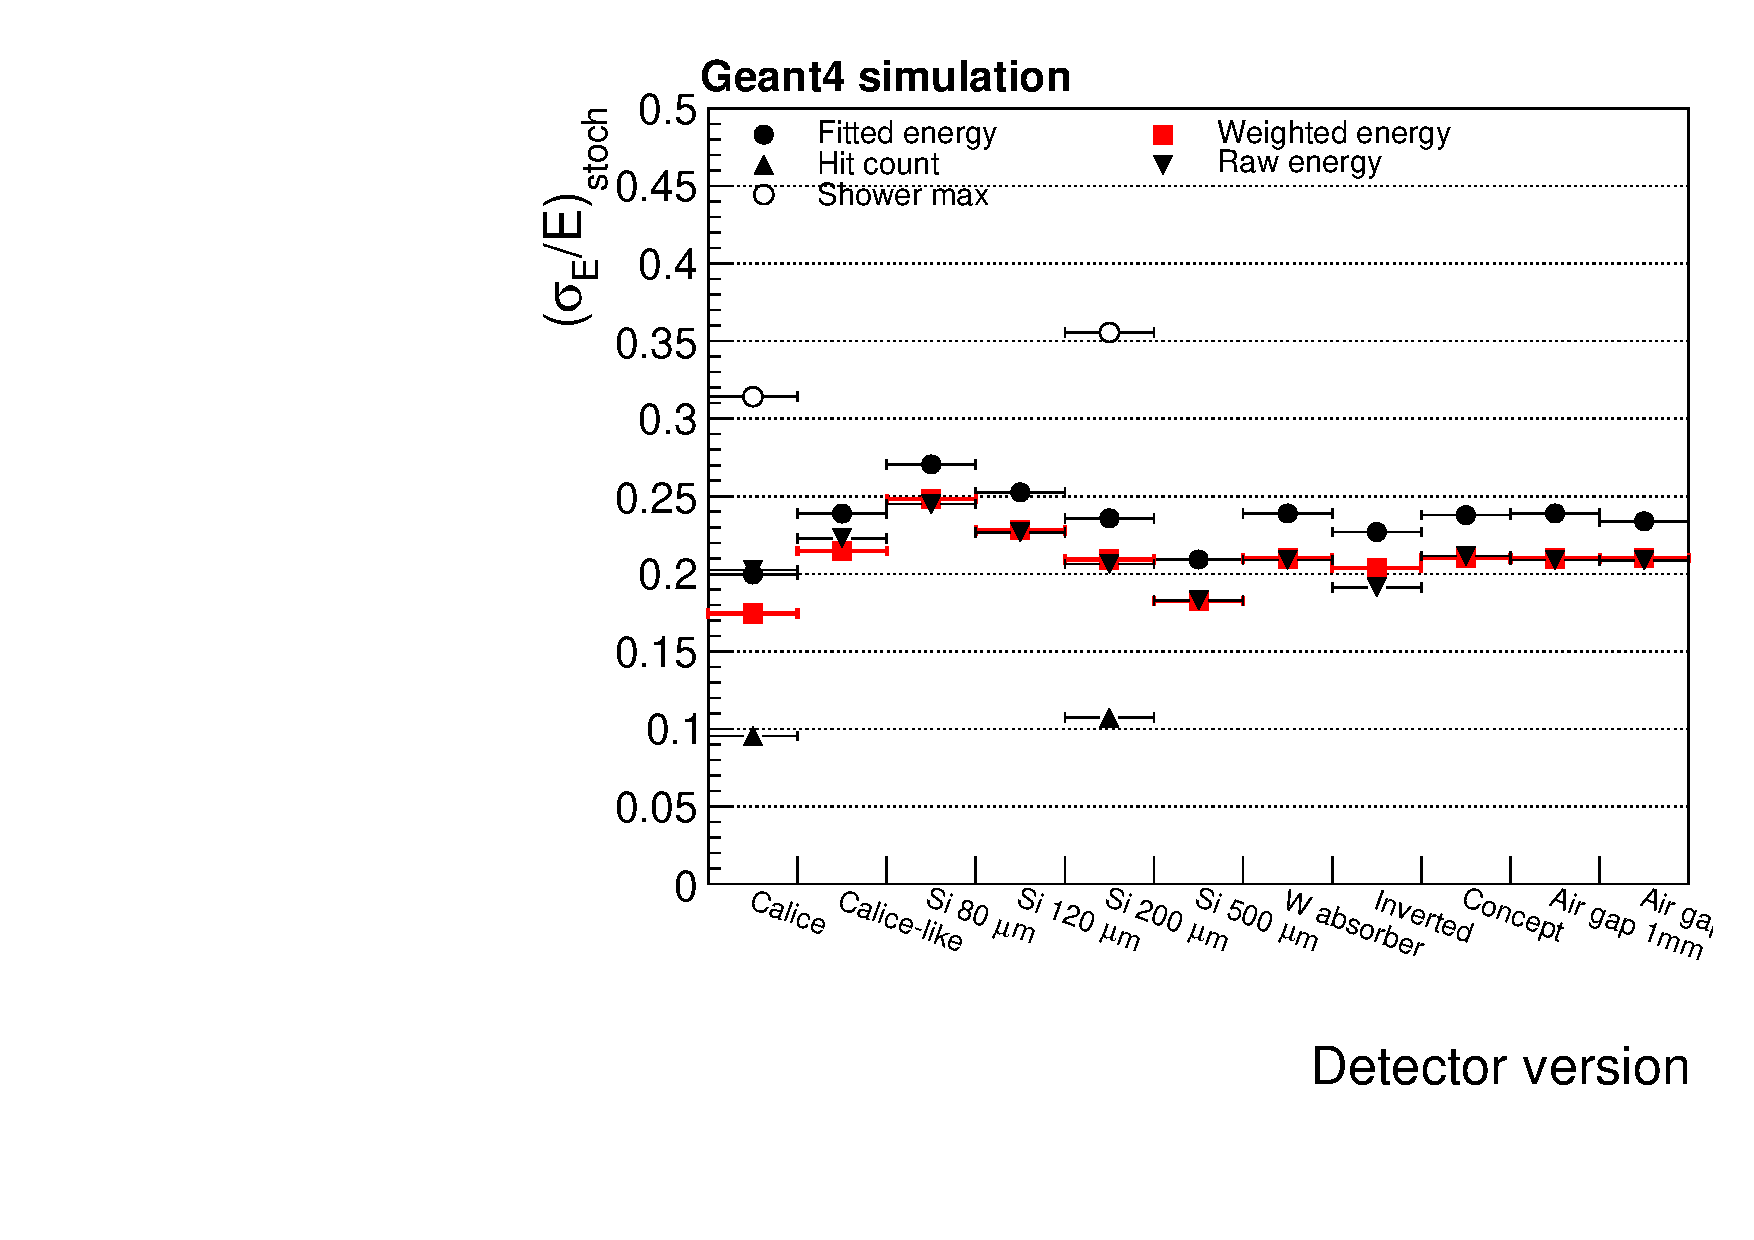
\includegraphics[width=0.75\textwidth]{figures/ResolutionSummary_stochastic}
  \caption{Summary of the fitted resolution curves to different
    setups and using different energy estimators. The constant term
    summary is shown on {\em top} while the stochastic term is
    shown on the {\em bottom}. }
    \label{fig:resol_summary}
  \end{center}
\end{figure}
% AM
\section{Digitisation}
\label{sec:digi}

The digitisation procedure is aimed at converting Geant4 SimHits into
reconstructed hits, i.e. reproducing what the electronics of the real
detector will do given an analogue signal, with a signal and a noise
component, passed through analogue-to-digital (ADC) convertors, with a
zero-suppression threshold applied to reduce the data volume, and
finally the calibration back to an energy.

Minimum ionising particles (MIPs) will deposit energy according to a
Landau distribution, whose maximum probable value can be used to
convert Geant4 energies into other relevant quantities. 

\subsection{The MIP signal}

The energy deposited by 50 GeV muons per $2.5\times 2.5$ mm$^2$ cells
is shown in figure~\ref{fig:muHits}. On the left the number of cells
with energy deposits are shown as a function of the layer, and on the
right the energy deposits for layers which have one and only one hit.

\begin{figure}[h!]
  \begin{center}
    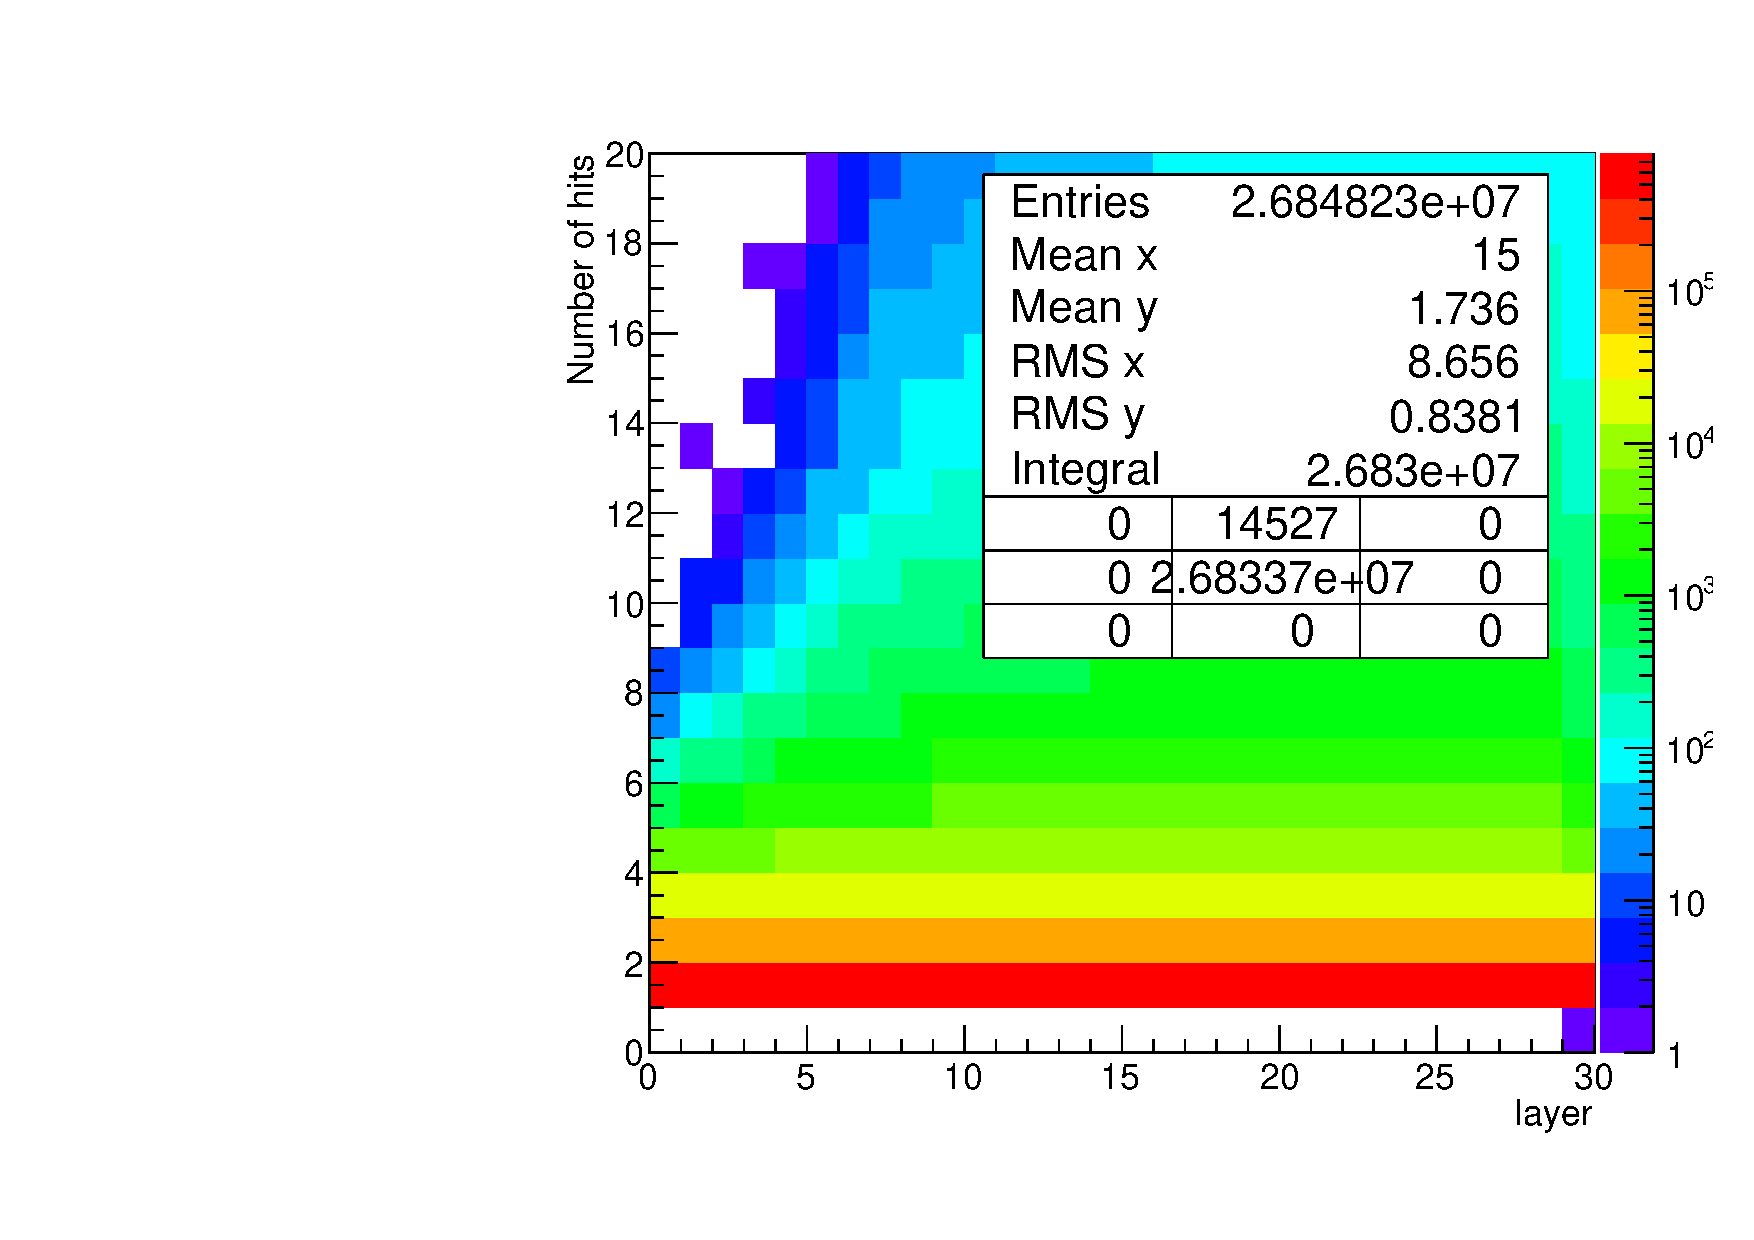
\includegraphics[width=\cmsFigWidth]{figures/mipHits.pdf}
    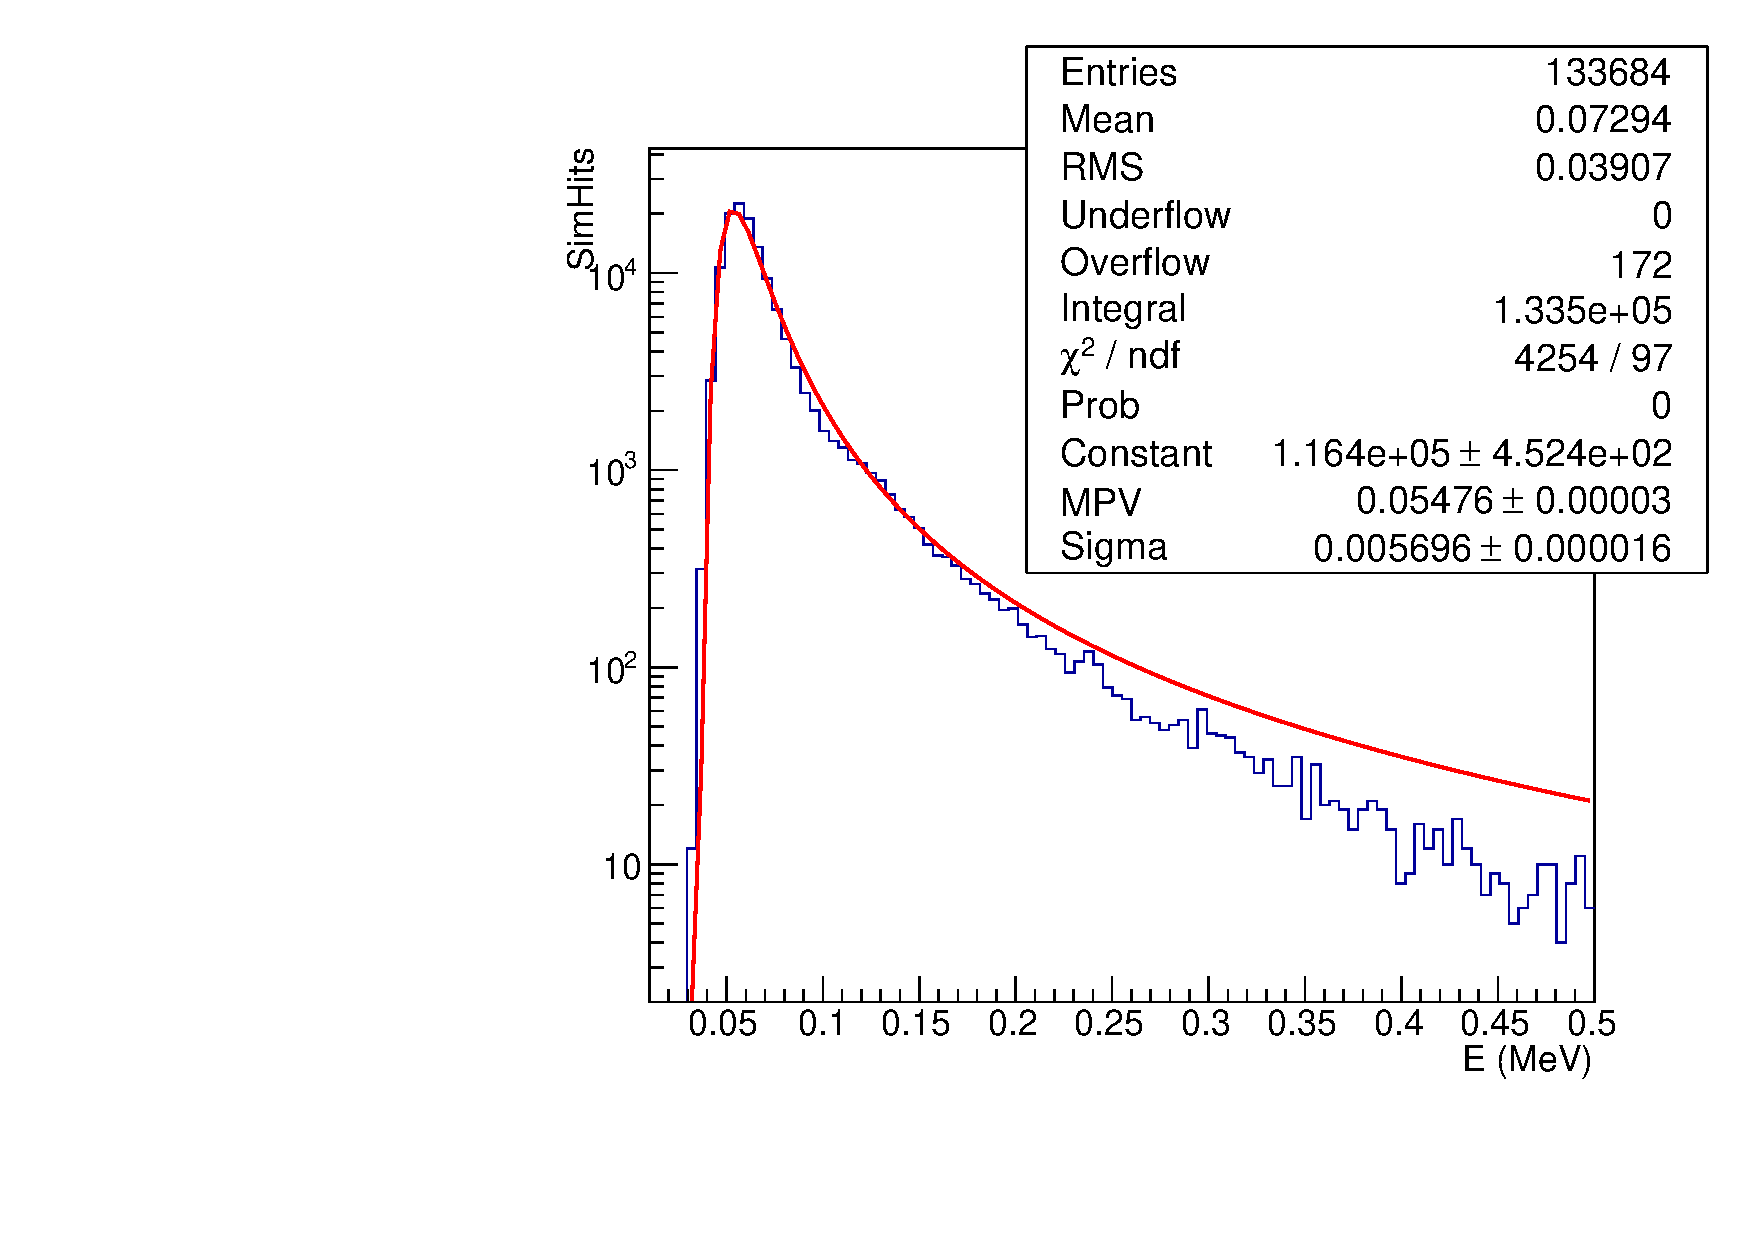
\includegraphics[width=\cmsFigWidth]{figures/mipDepositSel.pdf}
    \caption{}
    \label{fig:muHits}
  \end{center}
\end{figure}

The maximum probable value of the Landau gives the conversion factor
of $$1 \mathrm{MIP} = 0.0545 MeV$$ of energy deposited in Geant4.

\subsection{Electronics calibration and noise}

\subsubsection{MIP to electron conversion}

A MIP will typically create about 75 electron/hole pairs per $\mu$m of
Si. In 200$\mu$m of fully depleted Si, we expect hence about $\simeq
15000$ electrons.

\subsubsection{Dynamic range and MIP to ADC conversion}

The energy deposited by electrons in $1 \times 1$ cm$^2$ Si pads is
shown in figure~\ref{fig:hitE}, on the left for 100 GeV and on the
right for 500 GeV of incoming energy. The dynamic range of the
electronics should hence cover something from below a MIP, in order to
have a calibration peak, and about 1500 MIPs.

\begin{figure}[h!]
  \begin{center}
    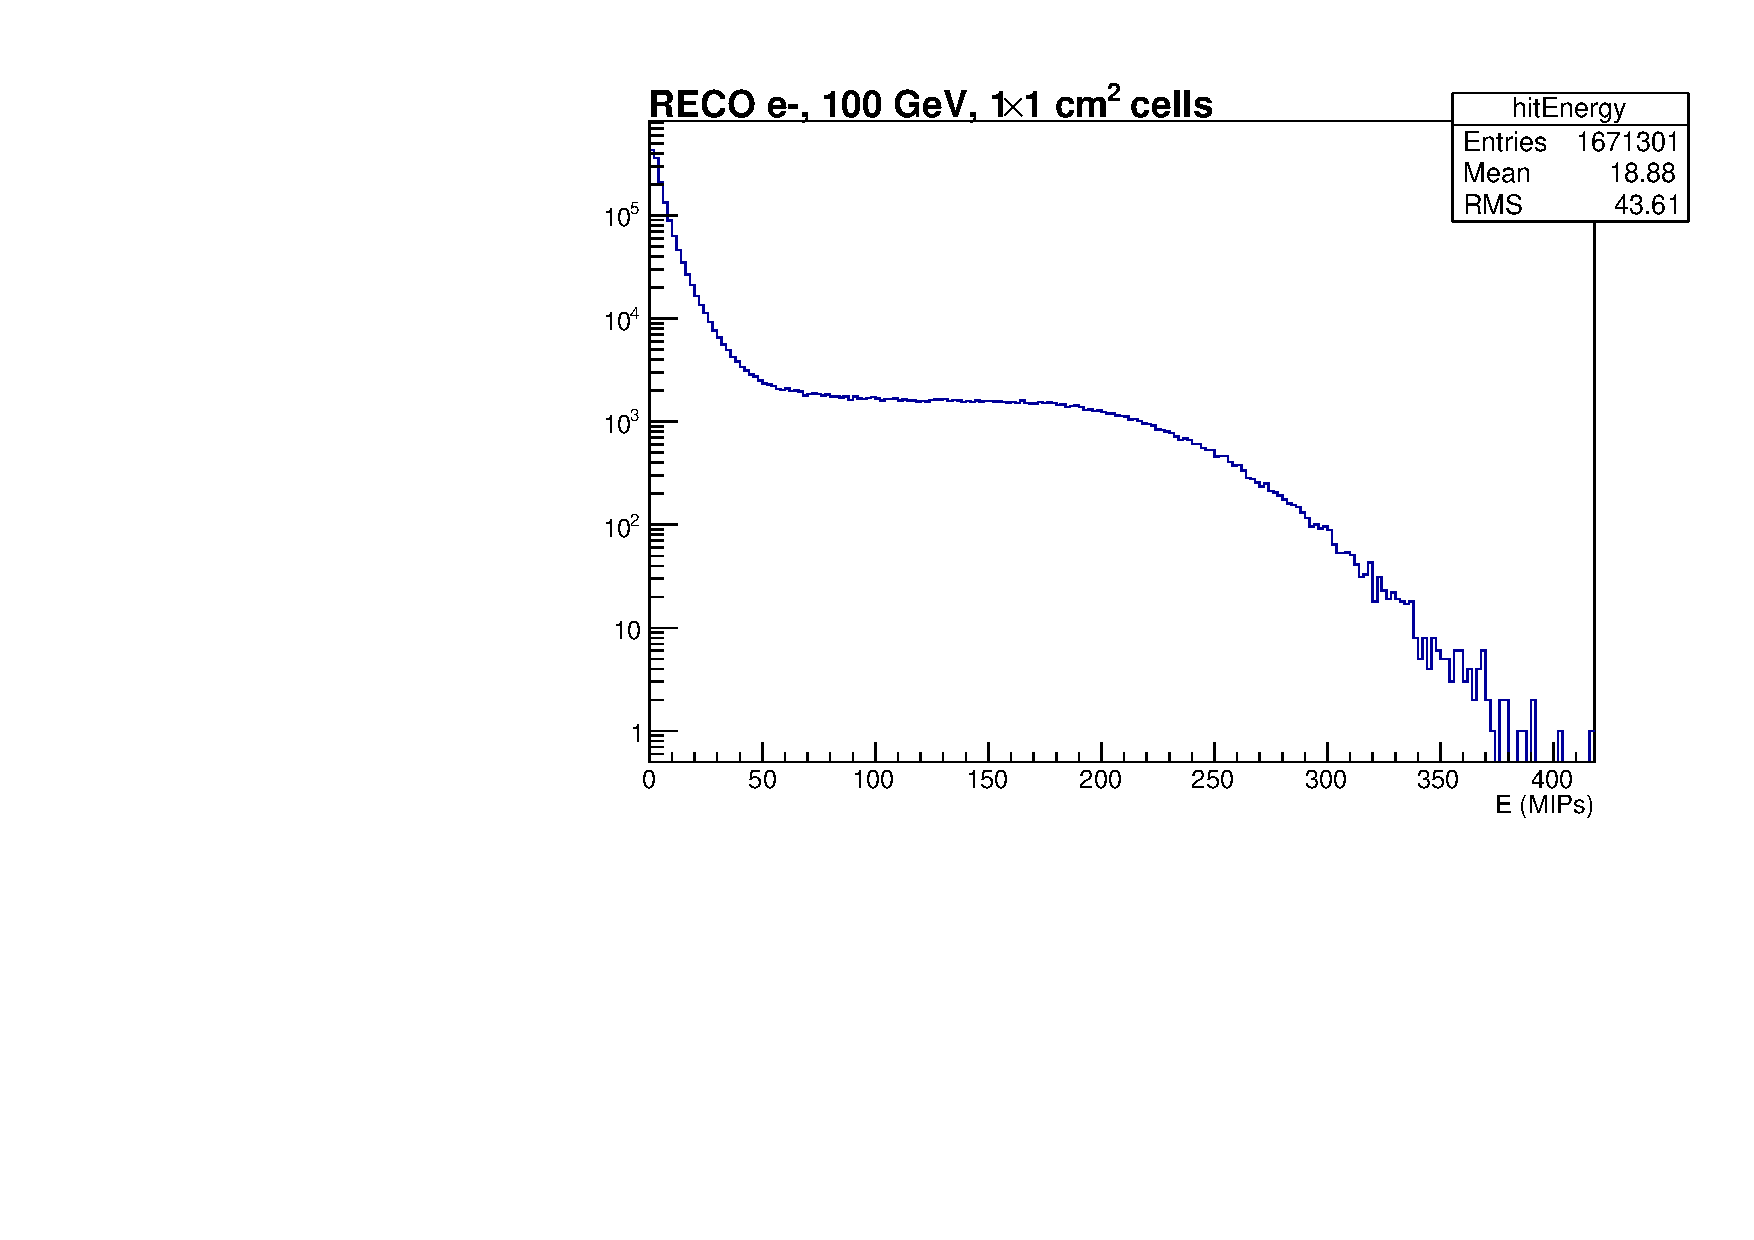
\includegraphics[width=\cmsFigWidth]{figures/HitEnergy_1x1_100GeV.pdf}
    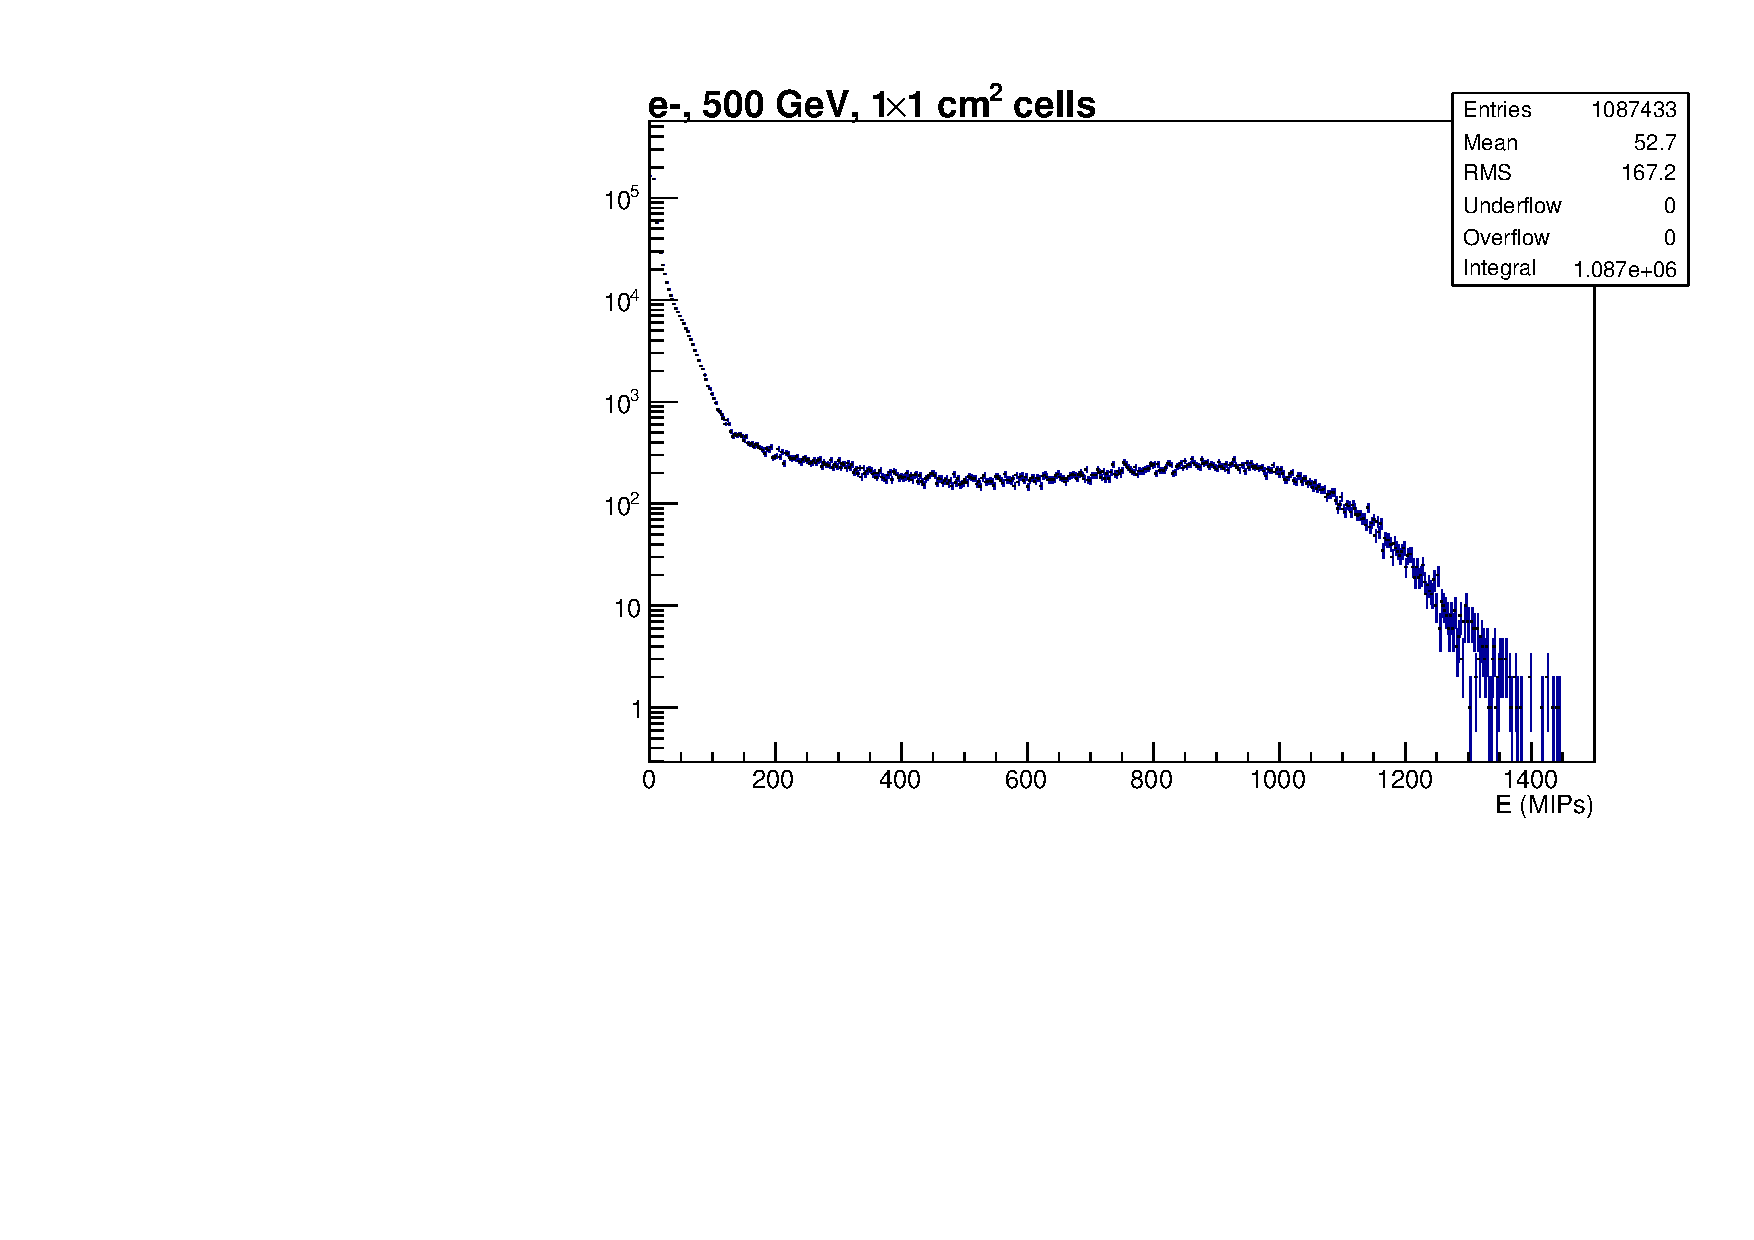
\includegraphics[width=\cmsFigWidth]{figures/HitEnergy_1x1_500GeV.pdf}
    \caption{Energy deposited by electrons per $1 \times 1$ cm$^2$ Si
      pads for 100 GeV (left) and 500 GeV (right) of incoming energy}
    \label{fig:hitE}
  \end{center}
\end{figure}

Three 10-bit ADCs are planned to be used:
\begin{itemize}
\item 10-bit ADC for a range up to 64 MIPs: so 16 ADC counts/MIP or 0.0625 MIP/ADC count.
\item 10-bit ADC for a range up to 1000 MIPs: so 1 ADC counts/MIP.
\item 10-bit ADC for a range up to 10000 MIPs: so 0.1 ADC counts/MIP or 10 MIP/ADC count.
\end{itemize}

The accuracy of the rounding scales as $\frac{x\mathrm{MIPs/ADC
    counts}}{\sqrt{12}}$, so 0.3 MIP for the 1 MIP/ADC count
conversion.

\subsubsection{Noise}

In the CALICE prototype, the signal/noise ratio was measured to be
around 9, so a noise level of about 0.13 MIP. Given this proposal uses
thiner silicon, we can expect a lower signal yield, so comparatively
higher noise. But the noise will decrease with smaller pad sizes, and
with cooling. Note that when using the conversion of 1 MIP / ADC
count, we can expect the noise level to be comparable or lower to the
digitisation accuracy.


\subsubsection{Procedure in software}

The procedure implemented in the standalone simulation is the following:
\begin{itemize}
\item Convert SimHits G4 energy (MeV) to MIPs.
\item Create collection of RecHits with the desired granularity. Baseline: $1 \times 1$ cm$^2$ pads.
\item Add noise in MIPs, included in empty cells.
\item Convert MIPs to ADC counts $\Rightarrow$ DigiHits.
\item Apply threshold: baseline = 5$\times$ noise.
\item Convert ADC counts back to MIPs $\Rightarrow$ RecHits.
\item All parameters are kept configurable for easy scanning.
\end{itemize}

\subsubsection{Impact on the resolution}

\FIXME{Add calibration and resolution curves after digi}
% All
\section{Performances}
\label{sec:perf}

\subsection{Ideal case}

\subsection{After digitisation, varying the parameters}

\subsection{Adding PU}
%
\section{Conclusion}
\label{sec:conclusion}


%% **DO NOT REMOVE BIBLIOGRAPHY**
\bibliography{auto_generated}   % will be created by the tdr script.

%% examples of appendices. **DO NOT PUT \end{document} at the end
%\clearpage
\appendix


%%% DO NOT ADD \end{document}!

